\documentclass[twocolumn,english,notitlepage]{article}
\usepackage[margin=2cm]{geometry}

% \setlength{\parindent}{0pt} % no indents

\usepackage{overhead} % Overhead is in a separate file

\title{Project 3}
\author{Anna Hjertvik Dåsen, Haakon Kværnmoen, et al.}

\date{\today}

\begin{document}

\twocolumn[
    \begin{@twocolumnfalse}
        \maketitle
        \begin{abstract}
            We integrated two LWTA algorithms, maxout and channel-out, with \texttt{tensorflow} neural networks and applied them to the MNIST and CIFAR-10 image recognition datasets. We visualised how these algorithms train specific pathways in its architecture, providing an opportunity to discern how information is encoded in the neural networks. A maxout neural network including dropout achieved a test accuracy of 51.28\% on the CIFAR-10 dataset, and a test accuracy of 50.69\% with a channel-out network with L2 weight penalisation.

            Furthermore, we created and analysed a dataset comprised of statistics from English Premier League football matches, and applied LWTA NNs in classifying results of the final matches 124 matches of the 2019/2020 season. With a maxout NN with dropout and L2 weight penalisation we got an accuracy of 58.06\%, and with a plain channel-out NN we got 54.84\%. Neither of these beat an ordinary dense NN with ReLU activation achieving an accuracy of 58.87\%. Here goes PCA results.
        \end{abstract}
    \end{@twocolumnfalse}
]

\tableofcontents

\section{Introduction}
The introduction goes here.

\begin{figure} [ht]
    \centering
    \includegraphics[width=\linewidth]{example-image-a}
    \caption{This is a figure}
    \label[figure]{int:fig:example}
\end{figure}

\section{Theory}
\comment{Suggestion: present tense, makes sense but might mess up some times H}\\
In this project, I thought we could use \verb|cleveref| to reference things like \cref{int:fig:example}.


Before we delve into to details of the theory section, it is useful to take a moment to define the quantities we will be dealing with. Let $\vec{y}$ denote a vector of a series of measured values $y_i$, $i\in 1, 2,\ldots, n$ at points $X$, where $X$ is a matrix where the rows $x_i$ correspond to the input values that produced the measurement $y_i$. For completeness, we refer to the columns of $X$ as $\vec{x}_a$, $a=1, 2,\ldots, p$.\footnote{Throughout this project, $a, b$ will always index the $p$ features for a model, and $i, j$ the $n$ data points.} Together, these form the dataset $\mathcal{D} = \cclosed{(y_i, x_i)}$. Another important set of values is $\vec{\theta}$ which contains the parameters that will define the model we will use to predict the data.

We will assume that the measurements $y_i$ are generated from an exact function $f(x)$ with stochastic noise $\epsilon$ added, such that $y_i = f(x_i) + \epsilon$. Throughout this project, we will assume that the noise to be distributed normally with zero mean and some standard deviation (std) $\sigma$; $\epsilon \distas \normal{0}{\sigma^2}$. Furthermore, we will assume that the noise between different measurements is independent and identically distributed (i.i.d.). Our job then is to model an $\hat{f}(x)$ that we want to be close to $f(x)$.
\comment{Copied this section from previous project, as it will be useful here too. Needs rewriting, -\Carl}
\comment{Also add somewhere: } \cite{Project1}.
\subsection{Gradient Descent Methods}
    \comment{This section might well be moved to method, it is not too theoretical. -\Carl}\\
    Optimisation of the parameters of the models we will be employing in this project is formulated as minimisation problems, with an associated cost function $C(\vec{\theta})$ to be minimised to find the optimal parameters.
    \subsubsection{Plain Gradient Descent}
        We will compare different variants of GD algorithm, starting first with the plain one. Assume the gradient of the cost function $C(\vec{\theta})$ w.r.t. the parameters $\vec{\theta}$ is well-defined on the entirety of our parameter space, and is calculable either analytically or approximated numerically\footnote{Now this is not always the case, e.g. with $L_1$-penalisation on the parameters.}. The idea is that the fastest direction to move in parameter space to reduce $C(\vec{\theta})$ is to follow the direction of $-\Nablatheta C(\vec{\theta})$. Plain gradient descent implements this idea iteratively, starting from an initial guess $\vec{\theta}_0$, finding the next point by
        \begin{align*}
            \vec{\theta}_{k} = \vec{\theta}_{k-1} - \eta \Nablatheta C(\vec{\theta}_{k-1}),
        \end{align*}
        where $k=1,2,\ldots,N$ for $N$ iterations, and $\eta$ is an introduced hyperparameter called the learning rate.

    \subsubsection{Adding Momentum}
        The simple GD can be fleshed out by giving the algorithm a sense of inertia, helping it continue to move in a certain direction. This combats tendency to oscillate around saddle points, for instance. It starts as earlier, but with the additional initialisation $\vec{p}_0 = 0$, finding $\vec{\theta}_k$ iteratively by 
        \begin{subequations}
            \begin{align}
                \vec{p}_{k} &= \gamma \vec{p}_{k-1} + \eta \Nablatheta C(\vec{\theta}_{k-1}), \\
                \vec{\theta}_k &= \vec{\theta}_{k-1} - \vec{p}_k,
            \end{align}
        \end{subequations}
        where $\gamma$ is a new hyperparameter characterising the memory of earlier gradients.

    \subsubsection{Stochastic Gradient Descent} 
        Stochastic Gradient Descent (SGD) is based on functions to minimise that are on the form $C(\vec{\theta}) = \sum_{i \in A} c_i(\vec{\theta}) + c_0(\vec{\theta})$ for $A=\cclosed{1,2,\ldots,n}$. This is often the case, as in MSE-scores, where a cost is associated with every observation $y_i$ separately. The idea of SGD is to avoid computing the gradient of the whole of $C$, but rather split it into mini-batches $C_k(\vec{\theta}) = \sum_{i\in A_k} c_i(\vec{\theta}) + c_0(\vec{\theta})$ for some subset $A_k \subseteq A$, and compute the gradient only on one of these smaller batches. This helps solve two problems: First, it makes the computational cost of calculating the gradient smaller, as we no longer compute the full one, and second, it adds a degree of stochasticity to the movement in parameter space since we no longer will follow the `true' gradient, which prevents getting stuck in local minima.

        SGD is done in so-called epochs, where we divide the full set $A$ into equally sized batches $A_k$, and do one GD iteration on every batch once. After this, $A$ is reshuffled and new mini-batches are drawn.

    \subsubsection{Improving Convergence Rate}
        \comment{Talk about learning schedules.}\\
        As stochasticity is added to the algorithm, the rate of convergence does slow down. As such, it would be nice to add algorithms that can adapt the learning rate $\eta$ in such a way as to increase the rate of convergence. The AdaGrad algorithm does this with the idea to use different learning rates along different directions in parameter space; i.e. use larger learning rates in flat directions, while keeping it small in steep directions. This is done by keeping a running sum $G_k$ of the outer product of the gradients $\vec{g}_k$ at the points $\vec{\theta}_k$, and use this to adapt the learning rate.
        \comment{I don't know whether to include the update rules in the \LaTeX-document, or maybe move them to method, or whatever. -\Carl}
        \begin{subequations}
            \begin{align}
                \vec{g}_k &= \Nablatheta C_k(\vec{\theta}_{k-1}) \\
                G_k &= G_{k-1} + \vec{g}_j \otimes \vec{g}_j \\
                \vec{\theta}_k &= \vec{\theta}_{k-1} - \eta G_k^{-\sfrac{1}{2}} \vec{g}_k
            \end{align}
        \end{subequations}
        where $\vec{v} \otimes \vec{u}$ denotes the outer product of two vectors $\vec{v}, \vec{u}$, and a matrix $m = M^{-1/2}$ is understood to the matrix satisfying $m^2 = M^{-1}$. Inverting and finding the root of $G_k$ comes at a computational cost, so we will employ the much cheaper version where we update \comment{Discussion note: mention uncorrelated features bettering this approximation, perhaps. -\Carl}
        \begin{align}
            \vec{\theta}_{k} = \vec{\theta}_{k-1} - \frac{\eta}{\sqrt{\diag(G_k)}+\epsilon} \circ \vec{g}_k,
        \end{align}
        where the arithmetic operations are understood to be element-by-element and $\vec{v}\circ \vec{u}$ represents the element-wise multiplication of two vectors $\vec{v}, \vec{u}$, and $\epsilon$ is a small number to avoid zero-division.
        
        The AdaGrad algorithm serves to tune the learning rate, and can be applied to gradient descent with momentum too. This gives the update rule
        \begin{subequations}
            \begin{align}
                \vec{g}_k &= \Nablatheta C_k(\vec{\theta}_{k-1}) \\
                \vec{p}_k &= \gamma \vec{p}_{k-1} + \eta \vec{g} \\
                G_k &= G_{k-1} + \vec{g}_j \otimes \vec{g}_j \\
                \vec{\theta}_k &= \vec{\theta}_{k-1} - \frac{\eta}{\sqrt{\diag(G_k)}+\epsilon} \circ \vec{p}_k
            \end{align}
        \end{subequations}

        Another way to adapt the learning rate to the parameter space `terrain' is found in the Root Mean Square Propagation (RMSprop) algorithm. Here we approximate a running average of the second moment of the gradient $\vec{s} = \expval(\vec{g} \circ \vec{g})$, then use this to scale the learning rate appropriately.
        \begin{subequations}
            \begin{align}
                \vec{g}_k &= \Nablatheta C_k(\vec{\theta}_{k-1}) \\
                \vec{s}_k &= \beta \vec{s}_{k-1} + (1-\beta) \vec{g}_k \circ \vec{g}_k \\
                \vec{\theta}_k &= \vec{\theta}_{k-1} - \frac{\eta}{\sqrt{\vec{s}_k}+\epsilon} \circ \vec{g}_k
            \end{align}
        \end{subequations}
        where again $\epsilon$ is a small number to avoid zero-division, and the arithmetic operations are understood to be element-wise. Here $\beta \in [0,1]$ is a new hyperparameter parametrising the rate at which previous gradients should inform the current average of the second moment.

        Finally, an algorithm which aims to combine RMSprop with momentum is Adam. Here we also keep a running average of $\vec{m} = \expval(\vec{g})$, i.e. the first moment of the gradient. Moreover, bias-corrected values are used in lieu of the `bare' estimates of the first and second moments, here denoted with hats. This ensures that a bias for low values of $\vec{m}_k, \vec{s}_k$ in early iterations with high $\beta$-values is avoided.
        \begin{subequations}
            \begin{align}
                \vec{g}_k &= \Nablatheta C_k(\vec{\theta}_{k-1}) \\
                \vec{m}_k &= \beta_1 \vec{m}_{k-1} + (1-\beta_1) \vec{g}_k \\
                \vec{s}_k &= \beta_2 \vec{s}_{k-1} + (1-\beta_2) \vec{g}_k \circ \vec{g}_k \\
                \vec{\hat{m}}_k &= \frac{\vec{m}_k}{1-\beta_1^k} \\
                \vec{\hat{s}}_k &= \frac{\vec{s}_k}{1-\beta_2^k} \\
                \vec{\theta}_k &= \vec{\theta}_{k-1} - \frac{\eta}{\sqrt{\vec{\hat{s}}_k}+\epsilon} \circ \vec{\hat{m}}_k
            \end{align}
        \end{subequations}


        \comment{Discussion notes: Adagrad accumulates G such that the learning rate becomes smaller with iterations --- AKA GD is `turned off'. -\Carl \\
        Not entirely true, rather learning rate stabilizes, I think. -\Carl}

    \subsection{Neural Networks}
        Artificial neural networks (ANN) are biologically inspired machine learning algoritms which can improve performance as they are exposed to data and without being programmed with any task-specific rules. In this project fully connected \textit{feed-forward neural networks (FFNN)} will be implemented. 
        \subsubsection{Structure}
        First a non-mathematical, intuitive introduction. 
        An ANN consists of an input layer and an output layer. Often the network will also have layers betweeen the input and output, called \textit{hidden layers}. In that case the neural network is referred to as deep. Each layer contains \textit{nodes} which are supposed to represent the neurons in a biological neural network, or rather their activation. In a fully connected neural network, all nodes in one layer are connected to all the nodes in the previous as well as the next layer. These connections, which represent the synapses, are referred to as \textit{weights}, and the sizes of the weights are the synaptic strength. Each node also have an activation \textit{bias} which says something about how easily activated that specific neuron/node is. See \cref{the:fig:Illustration_NN} for an illustration of a simple, deep artificial neural network. 
        \begin{figure} [ht]
            \centering
            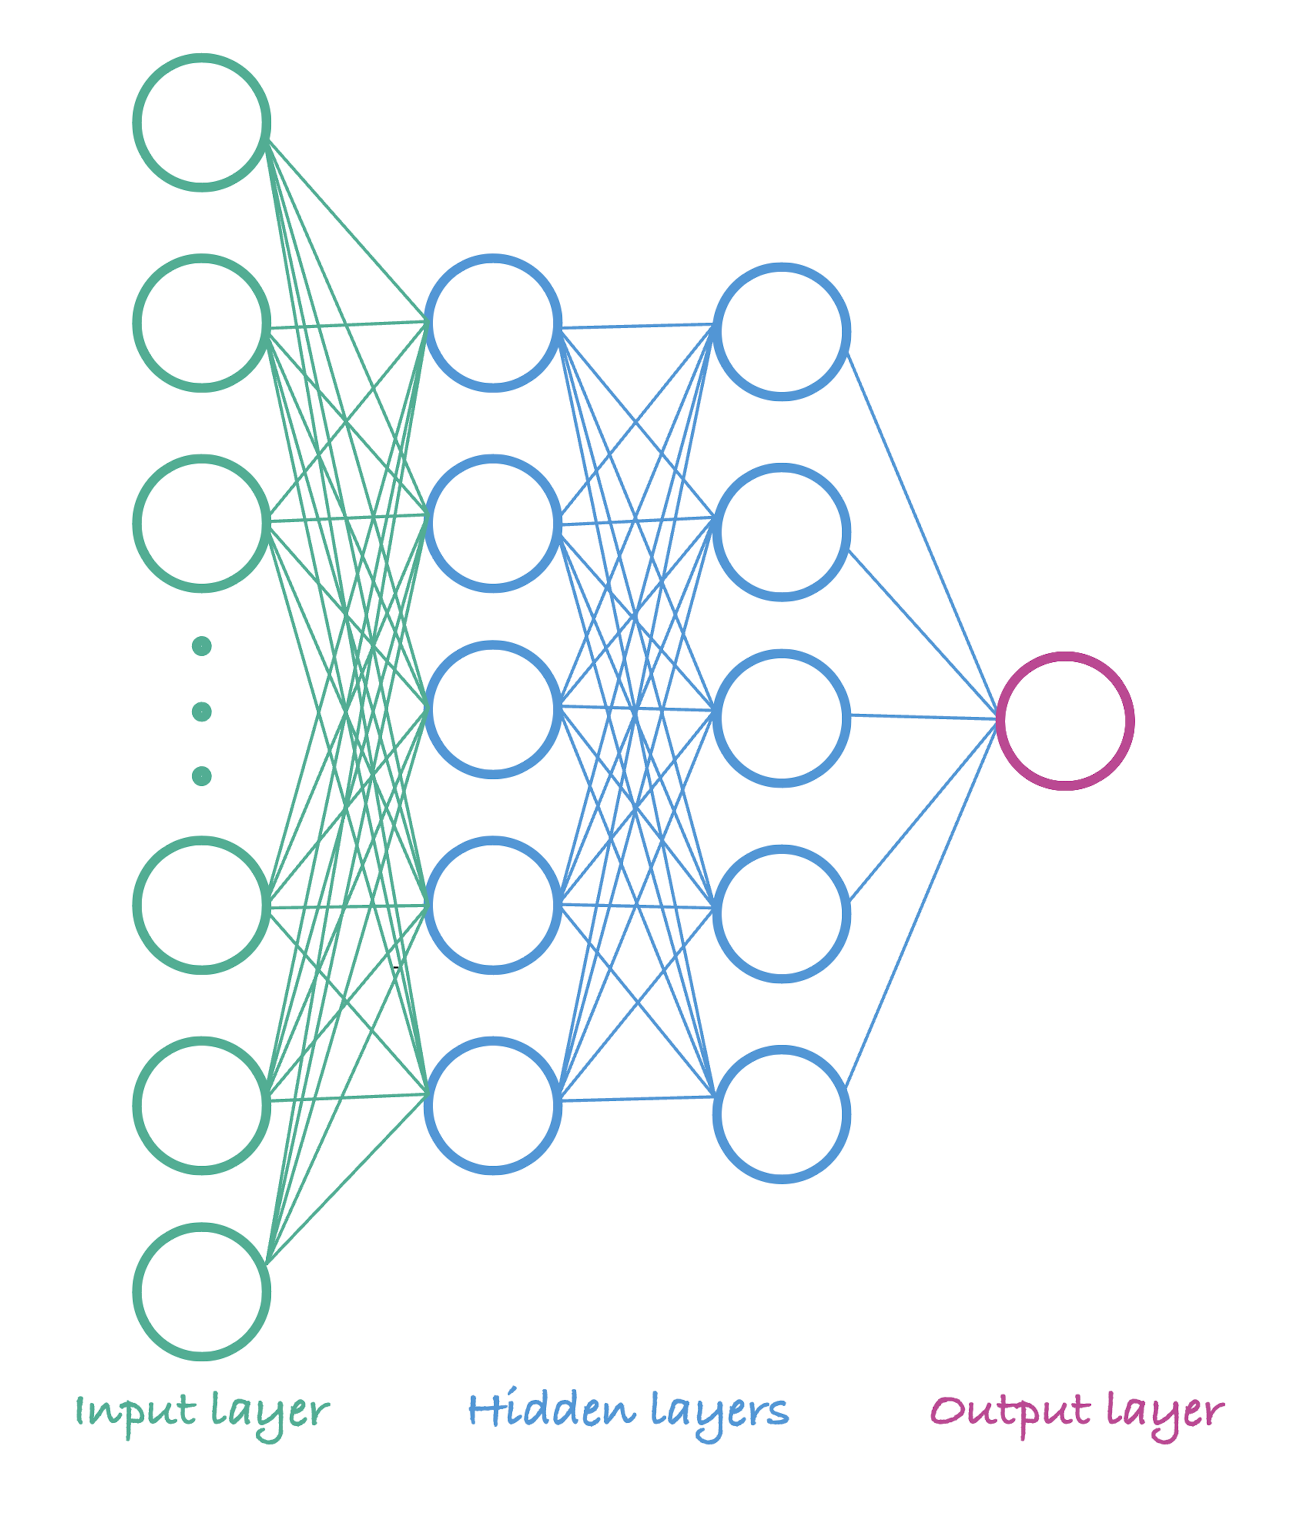
\includegraphics[width=.85\linewidth]{figs/Illustration_NN.png}
            \caption{Illustration of a simple deep neural network with an input layer, two hidden layer, and an output layer. The circles are the nodes and the lines between are the weights.}
            \label[fig]{the:fig:Illustration_NN}
        \end{figure}
        
        The nodes, weights and biases are all essentially just numbers, but following an algorithm for combinig these numbers creates an ANN. 

        \subsubsection{Feed Forward}
            \begin{figure} [ht]
                \centering
                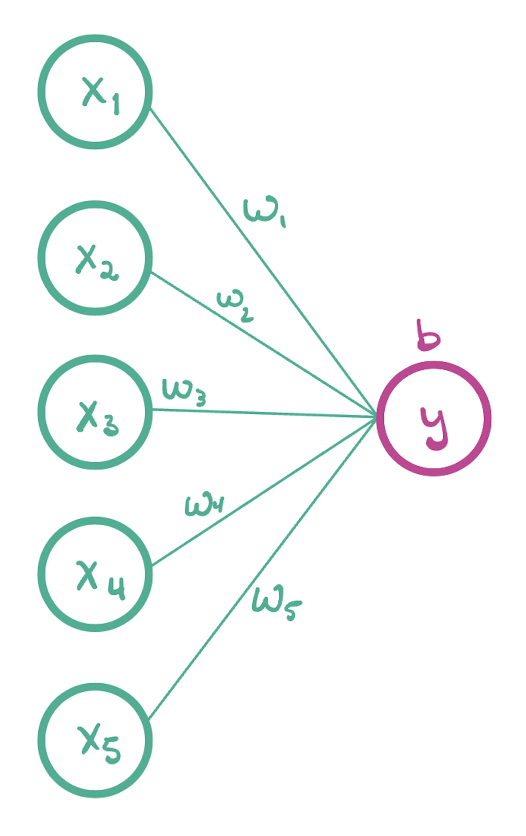
\includegraphics[width=.4\linewidth]{figs/Illustration_simple.png}
                \caption{Illustration of a simple neural network with an input layer, and an output layer consisting of one node.}
                \label[fig]{the:fig:simple_NN}
            \end{figure}
            The simplest of neural networks is the \textit{Feed Forward Neural Network(FFNN)} which, as its name implies, feeds activation from the input layer and forward through the network, eventually ending up in the output layer. Given a NN with only an input layer, and an output layer consisting of one node (see \cref{the:fig:simple_NN}), the output $y$ is then  
            \begin{equation}
                y=f\left(\sum_{i=1}^n w_i x_i+b\right)
            \label[eq]{the:eq:output}
            \end{equation} 
            where $x_i$ constitutes the input, $w_i$ are the weights corresponding to each input variable, and $b$ the bias of the output node. $f$ is called the \textit{activation function} and depends on the analysis being executed; e.g. regression, classification, etc. Each node has a corresponding activation function which defines the possible outputs of that node. The activation function closest to replicating the behaviour of a biological neuron is the heaviside function which yields either $0$ or $1$; firing or not firing. However, there are in some cases advantages of abandoning this biological model. Some other, and currently more used activation functions are: linear, sigmoid, relu, tanh, and leaky relu some of which are plotted in \cref{the:fig:introducing_acts}. \comment{See more on activation functions in appendix ref} 
            \begin{figure} [ht]
                \centering
                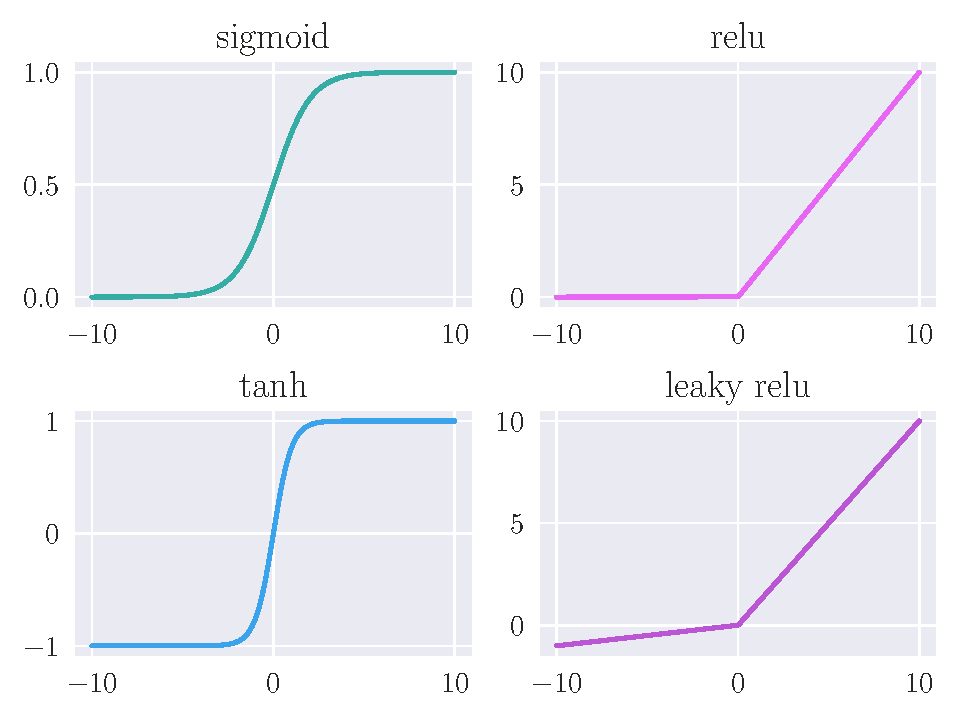
\includegraphics[width=\linewidth]{figs/introducing_acts.pdf}
                \caption{Plots of some commonly used activation functions.}
                \label[fig]{the:fig:introducing_acts}
            \end{figure}
            
            In the output layer the activation function constitutes what analysis the network does. E.g. a form of binary classification can be done by implementing the sigmoid activation function in the output layer, and for regression problems the linear function, $f(x)=x$, is implemented.
            It is normal that all the nodes in a layer have the same activation function $f$.    

            If we were to have a more complex neural network than the one from \cref{the:fig:simple_NN}, now also including hidden layers, $y$ (ref \cref{the:eq:output}) would be a node in the layer after the input. Each such node would have its own activation bias and would be connected with the input, or activation from the previous layer, through "unique" weights.  
        

        \subsubsection{Backpropagation}

    \subsubsection{Universal Approximation Theorem}

\subsection{Logistic regression}
    For comparison with our neural network we introduce maybe the most common classification method there is, \textit{logistic regression}. One might be confused by inclusion of the word \textit{regression} in the name of a classification method. This comes from preforming a fit to the \textit{log-odds} using a function linear in the input variables:
    \begin{align*}
        P(\vec{y}|X,\vec{\vec{\theta}}) = \prod_{i = 1}^{n} \sigma(X_{ia} \theta_a)^{y_i}[1-\sigma(X_{ia}\theta_a)]^{1 - y_i}
    \end{align*}

    \begin{align*}
        \log(\frac{p_{y_i}(x_i)}{1-p_{y_i}(x_i)}) = x_i^T \theta
    \end{align*}

    \begin{align*}
        P(\vec{y}|X,\vec{\vec{\theta}}) = \prod_{i = 1}^{n} \sigma(X_{ia} \theta_a)^{y_i}[1-\sigma(X_{ia}\theta_a)]^{1 - y_i} 
    \end{align*}

    \begin{align*}
        \msub{C}{BCE}(\vec{\theta}) &= -\log P(\vec{y}|X,\vec{\vec{\theta}}) \\ 
        &= - \sum_{i = 1}^{n} y_i \sigma(X_{ia} \theta_a) + (1 - y_i)[1-\sigma(X_{ia}\theta_a)]
    \end{align*}

    \begin{align*}
        (\grad_{\theta} \msub{C}{BCE})_b &= \sum_{i = 1}^{n} y_i [1 - \sigma(X_{ia} \theta_a) ] X_{ib} + -(1 - y_i)\sigma(X_{ia} \theta_a)X_{ib} \\
        &= \sum_i^n (y_i - \sigma(X_{ia}\theta_a)) X_{ib}  
        \pdv{\theta_b} \msub{C}{BCE} \\
        &= \sum_{i = 1}^{n} \left( (1 - y_i)\sigma(X_{ia} \theta_a) - y_i [1 - \sigma(X_{ia} \theta_a) ] \right) X_{ib} \\
        &= \sum_i^n (\sigma(X_{ia}\theta_a)- y_i) X_{ib}  
    \end{align*}

    \begin{align*}
        \nabla_{\vec{\theta}} \msub{C}{BCE}(\vec{\theta}) = X^T (\hat{\vec{p}} - \vec{y}) 
    \end{align*}

\section{Method}
Method here, in past tense.

We reference like this using \verb|cleveref|: \cref{int:fig:example_a}, \cref{theo:eq:newton2}.

\subsection{Datasets}
    \comment{Here we describe how we construct and prepare the dataset. -\Carl}

    \subsubsection{MNIST}
        A simpler test for our neural networks is the MNIST benchmark dataset. It consists of 60 000 training images and 10 000 testing images. Each image consists $28 \times 28$ pixels depicting handwritten number between 0 and 9. As such, the images are to be classified to one of the 10 categories of digits. Some examples of the images in the dataset are depicted in \cref{met:fig:MNIST}.
        \begin{figure}
            \centering
            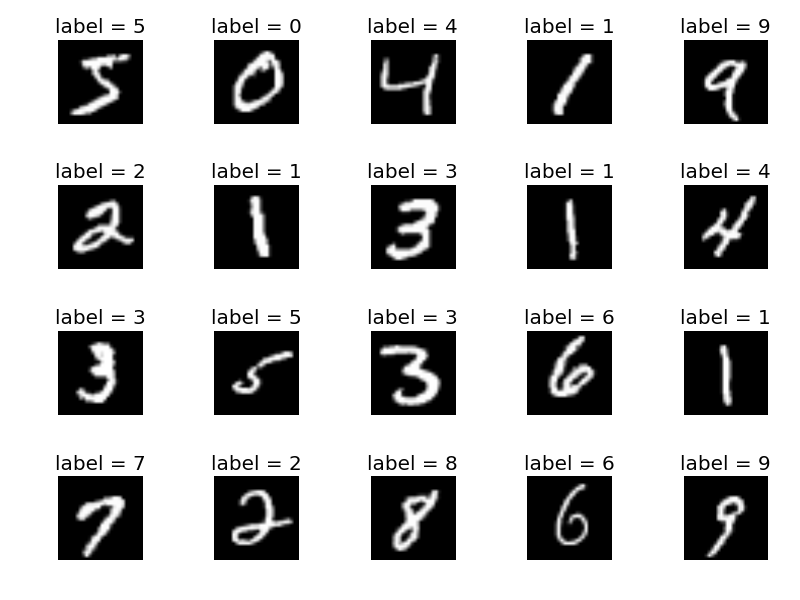
\includegraphics[width=\linewidth]{figs/MNIST_examples.png}
            \caption{20 example images from the MNIST dataset with their appropriate labels.}
            \label[fig]{met:fig:MNIST}
        \end{figure}

    \subsubsection{CIFAR-10}
        Initially, we applied our the LWTA NNs on the CIFAR-10 benchmark dataset for image recognition. This dataset consists of 60 000 images with $32 \times 32$ coloured pixels with RGB values, amounting to 3072 features per image. The images are divided into 10 categories, depicting one of either aeroplanes, birds, cars, cats, deer, dogs, frogs, horses, ships or trucks (see \cref{met:fig:CIFAR10}).

        \begin{figure}[ht!]
            \centering
            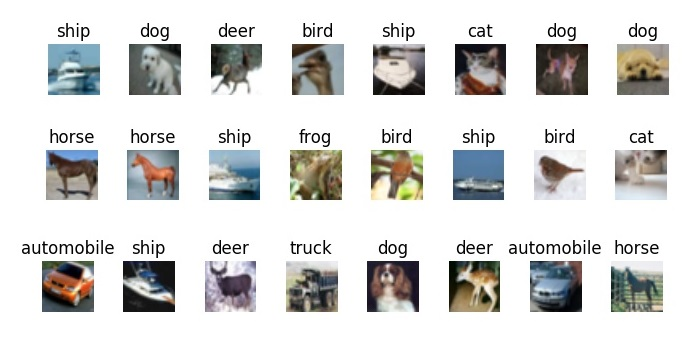
\includegraphics[width=\linewidth]{CIFAR10_examples.jpg}
            \caption{Examples of the images in the CIFAR10 dataset.}
            \label[fig]{met:fig:CIFAR10}
        \end{figure}

    \subsubsection{Premier League 2019 Season}
        \comment{The following is very draft-y. Will write it properly when my head is clear xD -\Nanna} 

        \comment{Maybe move some of this to intro? Not sure.}

        As well as for many other sports, data science is becoming more and more influential in the football industry~\citep{Herbinet2018}, both from the viewpoint of the club, e.g. in terms of choice of strategy or player acquisition and as seen by the odds market or the solely economically interested parties, be it e.g. club owners or league strategists, for making sure they benefit from the industry by possessing valuable data and powerful prediction algorithms. Analysts working in the larger leagues have access to technology that gives them more complex data than the main match events such as number of goals scored or corner given. For instance, a group on football analysts will most likely measure a team's or player's performance through metrics like expected goals (xG) or the number of passes allowed per defensive action (PPDA). The former is a very much used measure in football, but the algorithm behind it is not universal. In the European Premier League (EPL), one may follow live updates of the xG's for two opposing teams during their clash on several sites, however, the exact measurement will be dependent on the xG model the site uses.
        
        For the biggest football league in the world, the bookmakers tend to keep the most interesting data to themselves, as do the clubs' data science teams \citep[Ch. 15]{Soccermatics}. However, being the most-watched sports league in the world, the public datasets form EPL are reliable and usually uncorrupted, and one can retrieve quite detailed match data from decades ago.

        The EPL is the primary division for men in the English football league system. 20 teams participate each season, three of which newly promoted from the English Championship. 
        
        %By the end of the season, three teams are necessarily relegated to this 

        The challenges in collecting data and the time scope of this project compelled us to keep the purpose simple and ambitions somewhat low. In particular, we aim to foresee the outcome of a league match in EPL season 19/20 with a dataset as shown in \comment{some figure (work in progress)}. After preprocessing stats from various sources, our dataset contains information about the ten league matches in each game week following the first one, but from the perspective of each team, giving $ 10 \times 37\times 2 = 740$ data points. We used the games from the first $\sfrac{5}{6}$ part of the season, not counting the 10 opening matches, for training, corresponding to 308 games. The remaining final games (62 games, last $\sfrac{1}{6}$ part of the season) was reserved for testing. 
        All in all, we had 616 training data points and 124 testing data points.
        
        The choice to look back only one league game for one team was due to a great ease in the data acquisition process. Trying to predict the full time result is a much more comprehensive task than to classify the outcome for a team as win (W), draw (D) or loss (L).

        Another important simplification we made concerns the promoted teams. As these teams did not participate in EPL by the beginning of 2018, we (quite naively) assumed that their previous season team profile corresponds to that of the average lower quartile of that season's table. \comment{(Ouf heavy sentence)} 

        

        




    \subsubsection{Data Preparation}
        \comment{Describe preprocessing of data, i.e. scaling etc. -\Carl}
        \comment{Data splitting \Anna}
        To train and evaluate our models we implemented the relevant data and as in our previous projects we split it in training data ($\sfrac{5}{6}$ of the data) and testing data ($\sfrac{1}{6}$ of the data) \citep{Project1, Project2}. When tuning the architecture, we further split the training data into a tuning set and a validation set used for monitoring overfitting, implementing early stopping with $p=5$. We used a split of $\sfrac{3}{4}$. See \cref{the:fig:illustration_data} for illustration of the data splitting. 

        \begin{figure}[]
            \centering
            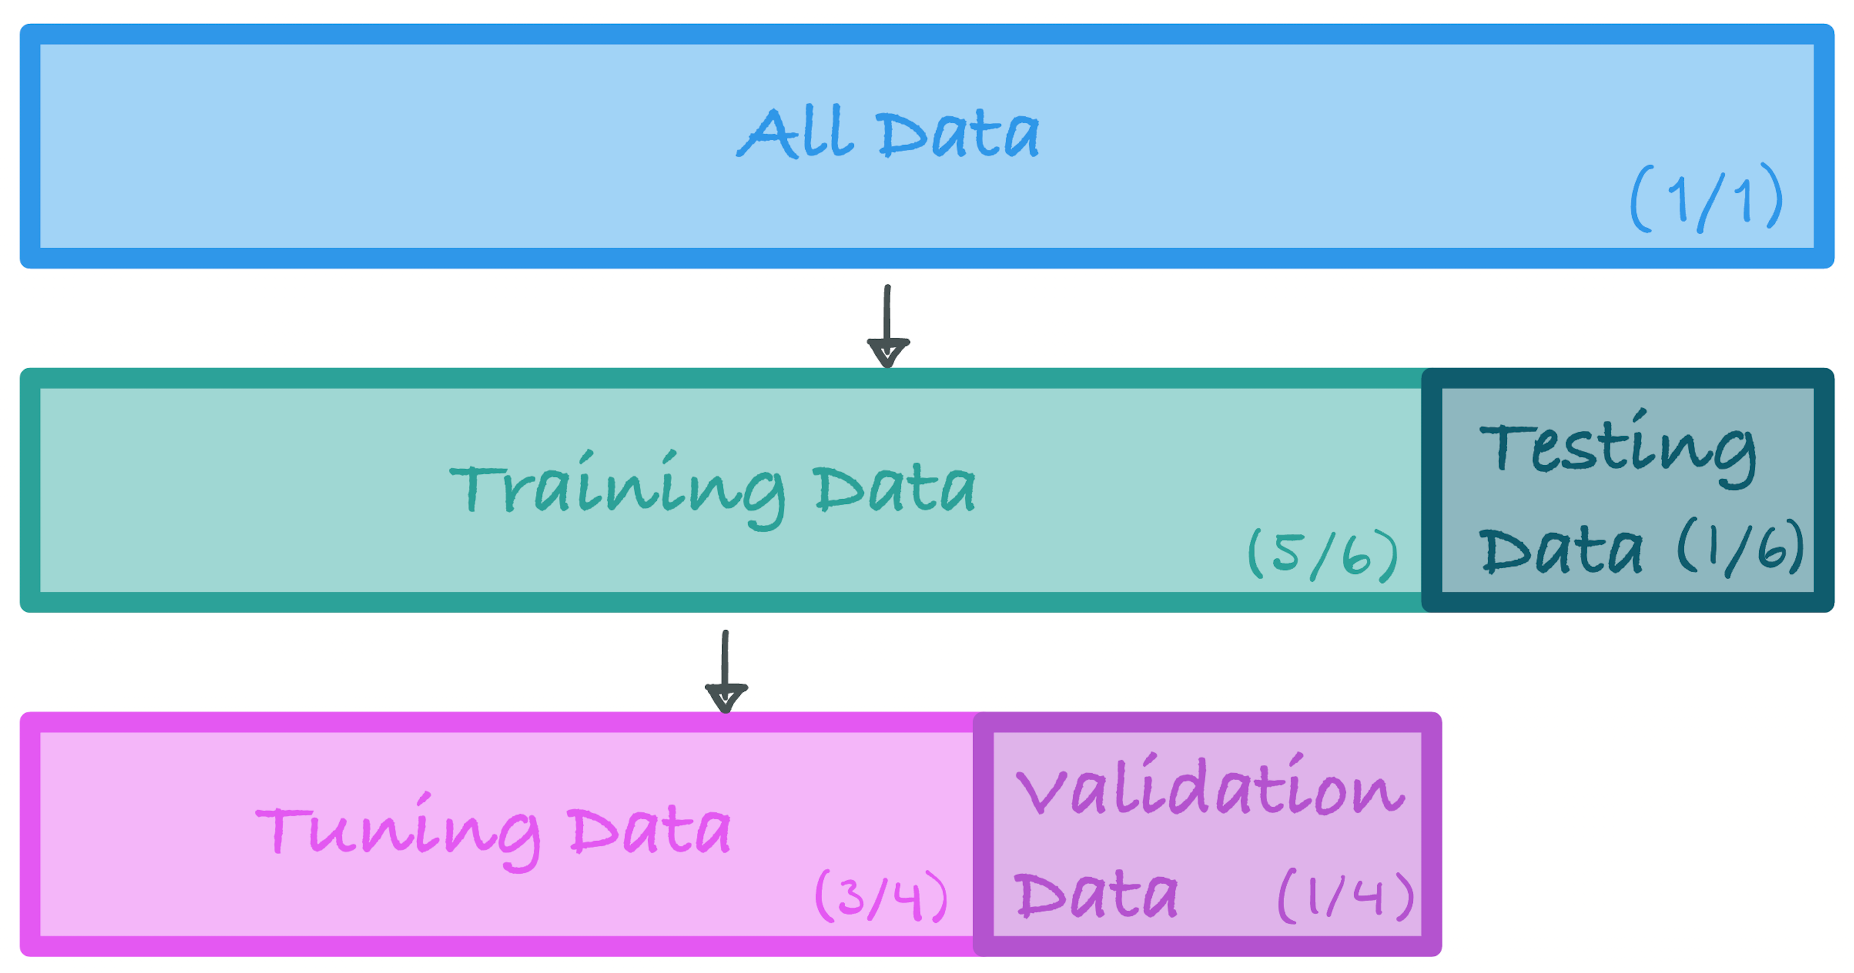
\includegraphics[width=.9\linewidth]{illustration_data.png}
            \caption{Illustration of data splitting.}
            \label[fig]{the:fig:illustration_data}
        \end{figure}

    \subsubsection{PCA}
        \comment{Could perhaps be part of data preparation \Anna} Before being subject to the principal component method, the Premier League data was z-score normalised, centring the mean around zero, with unit variance. This ensured that no single feature with a relatively large variance would dominate any of the principal components. The principal components found created a new basis for the data, and had similar shape as the original features (they were linear combinations of them). Extracting the first few of these yielded the most important components, used for further analysis. For all principal components we found the explained variance, which is the ``amount'' of variance accounted for by the principal component in question. In order to make an attempt at reducing the dimension of the problem, we found the number of principal components necessary in order to explain 99 \% of the variance of the original features. \comment{Hmmm more/other/change idk \Johan} The Premier League dataset was the only dataset on which we performed PCA analysis. 


\subsection{Neural Network training}

    \subsubsection{Initialisation of the Neural Network Weights}
        It is important to take care when initialising the weights and biases of a neural network to ensure fast convergence during training. We initialised the weights according to the He algorithm~\citep{He}. In our case it meant initialising the weights of node $i$ in layer $\ell$ by the distribution
        \begin{align}
            w^\ell_{ij} \distas \normal{0}{\sqrt{2/\hat{n}}},
        \end{align}
        where $\hat{n}$ is the number of inputs to the layer. The biases were all initialised to zero.

    \subsubsection{Optimisation Algorithm}
        When optimising the cost function of our problems we built on what we found in \citep{Project2}, using stochastic gradient descent with a batch size of 32. We used the Adam algorithm with hyperparameters $\beta_1 = 0.9$, $\beta_2 = 0.999$ and a learning rate $\eta = 0.001$. These hyperparameters were not tuned in any of our searches. The number of training epochs was decided with early stopping termination criterion. This means monitoring the loss of the network on a validation dataset after each epoch of training, and stopping the training if there is no improvement after a number of epochs $p$, called the \textit{patience}.

        All the datasets used pose classification problems with 3 or 10 categories. The cost function we used for optimisation was the standard categorical cross-entropy. Predicting probabilities $\vec{p}_c$ for the outcome being in category $c$ for the datapoints $\vec{y}_c$, with $n$ datapoints, the categorical cross-entropy is given by
        \begin{align}
            \mathcal{L}(\tilde{y}) = \sum_{i=1}^n \sum_{c \in \mathrm{categories}} y_{i,c} \log\pclosed{p_{i,c}}.
        \end{align}

        \comment{Discussion note: Early stopping prevents overfitting. -\Carl}

    \subsubsection{Regularisation}
        The first method we applied to combat overfitting was to add a L2 penalisation term to the kernel weights of the layers, as was done in \cite{Project2}. This adds a term to the cost function penalising large weights, and is parametrised with a hyperparameter $\lambda$, whose size is proportional to the penalisation.

        A problem that can occur in LWTA layers is when the weight of a certain input to one of the nodes of a group becomes much larger than those of the other nodes in the group, resulting in the output of the group being dominated by a single node and a single input. This can result in overly local training, perhaps even of a single node and a single weight. A common technique to combat this is to add a dropout layer before and/or after the LWTA layer. The dropout layer randomly sets elements of its input vector to zero, according to a dropout rate, before passing it on to the next layer. This means that the nodes in a group cannot solely lean on one specific node or input, and forces pathways in the network to not learn specific trends `too much'. As such, it prevents overfitting, and can be seen as a regularisation method. The dropout layers are only active during training, and do not drop any activations at inference time. The effect of dropout on a LWTA network is illustrated in \cref{met:fig:dropout_network}.

        \begin{figure}
            \centering
            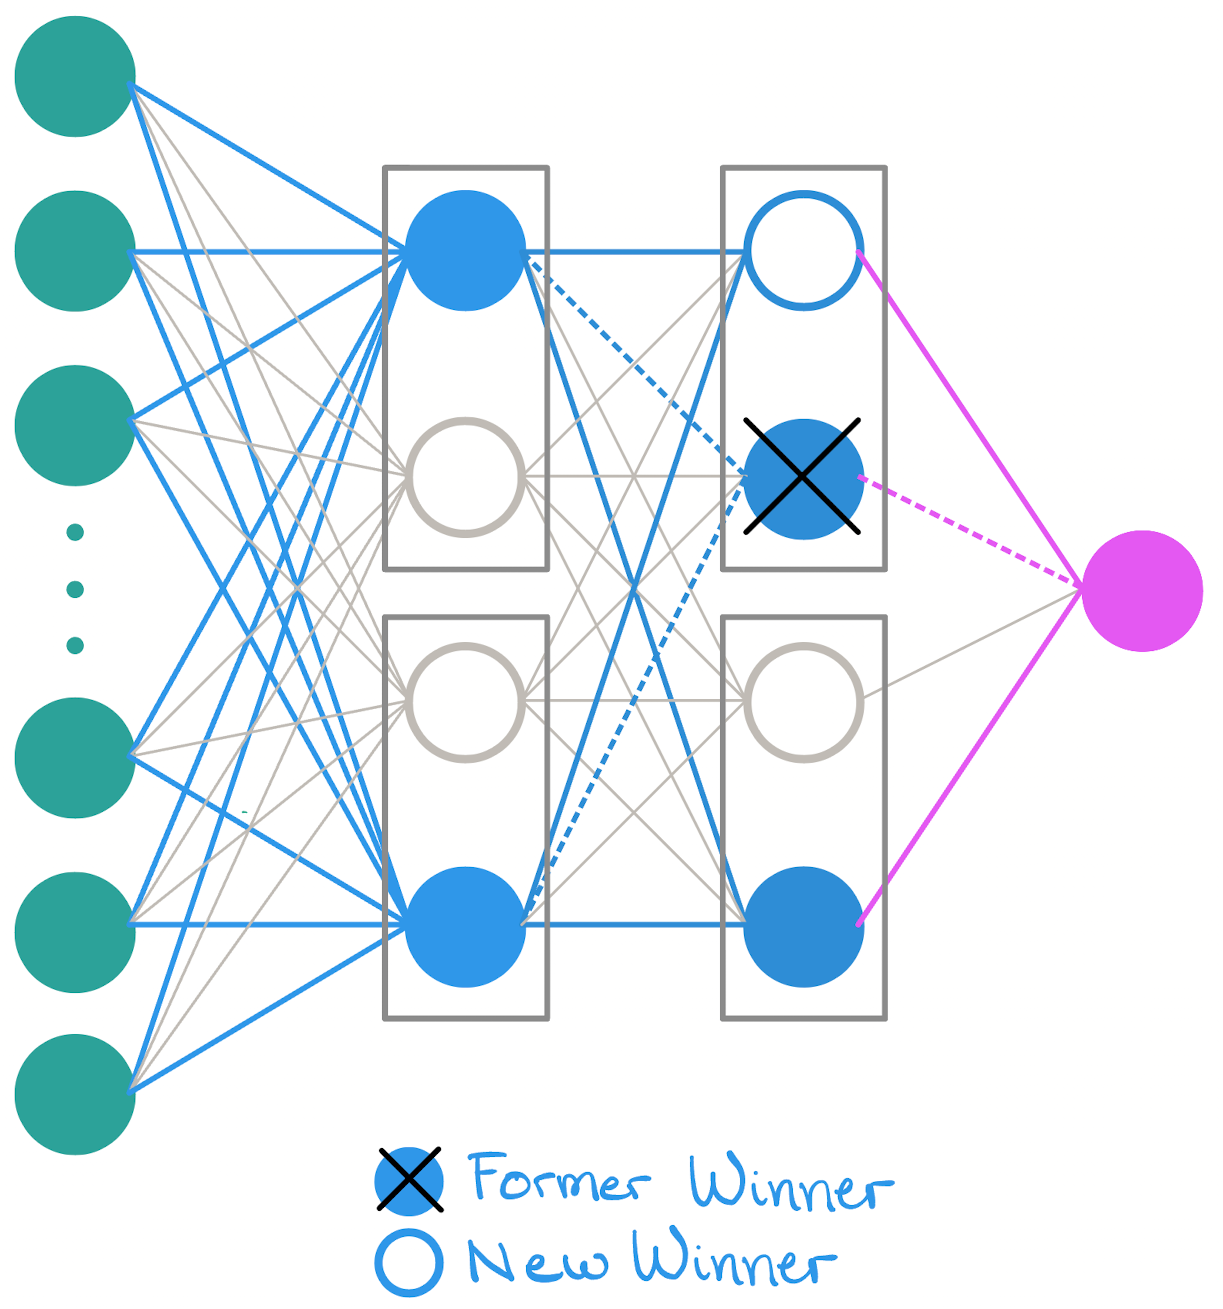
\includegraphics[width=.9\linewidth]{figs/illustration_dropout.png}
            \caption{An illustration channel-out neural network with a dropout added to the first channel-out layer. Only the lower group in the first hidden layer is trained.}
            \label[fig]{met:fig:dropout_network}
        \end{figure}

        When adding dropout to our networks, we did so with between every layer with the same dropout rate. This includes dropout on the input layer.


\subsection{Visualising Pathways}
    A good place to start with LWTA networks is to take a look at what actually happens during inference. We fitted a channel-out network on the full training MNIST dataset with three layers, 8 nodes in each and 4, 2 and 4 groups respectively in each network. This was done with a dropout rate of $0.125$, ridge penalisation added with $\lambda = 0.01$, and early stopping with $p=5$. We then plotted the pathways that were activated when inputting 200 test images depicting zeros, ones, fours and fives.

\subsection{Architecture tuning}
    To see what kind of network architectures were interesting and useful when applying to the datasets at hand, we tuned the architecture using the \textit{hyperband} search algorithm \citep{Hyperband}.

    We searched with a variable number of hidden layers between 2\textendash5, a number of nodes in the layers between 8\textendash64 in powers of 2, and a number of groups in the layers between 4\textendash32, again in powers of 2. When hyperparameters were chosen such that the number of groups was equal to or greater than the number of units in a layer, we set the layer to be a dense layer with the specified number of units, but added a ReLU activation to the output.

    \subsubsection{Hyperband Search}
        The hyperband search algorithm serves as a way to tune the hyperparameters of a model in a way such that more computing resources are dedicated to more promising areas of the hyperparameter space. It is based on the \textit{successive halving} algorithm, in which a finite budget $B$ (i.e. number of training epochs) is divided evenly between $n$ randomly sampled points from the hyperparameter space. These hyperparameters are then used to build $n$ models that are trained according to $r = B/n$ allocated resources on a tuning dataset, and their loss evaluated on a validation dataset, passing on the $k$ top performing models.\footnote{Usually the top half of the is passed on, as the algorithm name would indicate.} 
        These $k$ models are then trained further, with a new $n=k$ and consequently more resources $r$. This halving is then repeated until there is one model remaining. As hyperparameter points are discarded ($n$ decreases), the amount of allocated resources $r$ increases; meaning the more promising hyperparameter points are allotted exponentially more resources.

        This introduces a trade-off in the division of the resources $B$; sampling a larger number of hyperparameter points $n$ leaves less resources $r$ for exploring each point. The hyperband algorithm aims remedy this by doing a grid search of different values of $n$ and smaller resource allotments $r$. For each value of $n$ and $r$, the successive halving is performed, and the best preforming model is found. In the end, models that perform better deeper into the training will be found, but many hyperparameter points will have been explored.

        Hyperband takes two hyper(hyper)parameters, $R$ indicating the maximum amount of epochs of training for any single hyperparameter point, and a factor $\eta$ which is the reciprocal of the fraction of points that are passed on during each halving.

        \comment{$R=30$, $\eta=3$ gives $27+12+6+4 = 49$ hyperparameter points explored.}

        % \begin{algorithm}
        %     \caption{Hyperband search algorithm}
        %     \begin{algorithmic}[1]
        %         \Procedure{Hyperband}{$R, \eta$}
        %             \State $\msub{s}{max} \gets \floor{\log_\eta(R)},\quad B \gets (\msub{s}{max}+1) R$
        %             \For{$s \in \cclosed{\msub{s}{max}, \msub{s}{max}-1, \ldots, 0}$}
        %                 \State $n \gets \ceil{\frac{B}{R} \frac{\eta^s}{(s+1)}},\quad r \gets R\eta^{-s}$
        %                 \State $T \gets \mathtt{get\_hyperparameter\_configurations}(n)$
        %                 \For{$i \in \cclosed{0, \ldots, s}$}
        %                     \State $n_i \gets \floor{n \eta^{-i}},\quad r_i \gets r \eta^{i}$
        %                     \State $L \gets \cclosed{\mathtt{fit\_then\_eval\_val\_loss}(t, r_i): t\in T}$
        %                     \State $T \gets \mathtt{top\_k}(T, L, \floor{\sfrac{n_i}{\eta}})$
        %                 \EndFor
        %             \EndFor
        %         \EndProcedure
        %     \end{algorithmic}
        % \end{algorithm}

    \subsubsection{CIFAR-10}
        On the CIFAR-10 dataset, we tuned using 1 hyperband iteration with a maximum number of epochs $R=30$ and $\eta=3$. We used early stopping with $p=5$ to terminate the training. After finding best network architectures, we fitted them on the full training dataset, evaluating their accuracy on the test dataset. We used early stopping with $p=10$ during this training.

        When adding dropout we used a dropout rate of $0.1$, and with Ridge penalisation we used $\lambda=10^{-4}$.

    \subsubsection{Premier League Dataset}
        With the smaller Premier League dataset, we could afford 3 full iterations of the hyperband search with a maximum number of epochs $R=150$ and again $\eta=3$. Again, we used early stopping during the tuning, with $p=15$. After finding the top-performing architectures, we trained on the full training set with early stopping with $p=30$.

        When adding dropout we used a dropout rate of $0.25$, and with Ridge penalisation we used $\lambda=10^{-4}$.


\section{Results}
\comment{Suggestion: past tense}\\

\subsection{Gradient Descent Analysis}
    First we looked at our library of gradient descent methods to figure out what and how they worked. This with the goal of finding a descent recipe for optimising our neural networks down the line.
    
    \subsubsection{OLS Optimisation}
        All plots regarding the optimisation of the OLS cost function are found in \cref{res:fig:lrates}. The best MSE scores and learning rates are tabulated in \cref{res:tab:OLS_MSEs}. We found that the none of the algorithms come really close to the analytical OLS solution, found by matrix inversion, with a validation MSE of $0.1176$. The best performing algorithms were SGD with Adam (MSE $0.1660 \pm 0.0018$), SGD with momentum (MSE $0.1729 \pm 0.0022$) and GD with momentum (MSE $0.1775 \pm 0.0026$).

        In \cref{res:fig:lrate1} we see that both the non-stochastic and stochastic algorithms performed better when momentum was added, which helped avoid local minima to converge faster and prevent exploding gradients. Generally, the stochastic algorithms had tighter confidence intervals, signalling that they are not as sensitive to the initial conditions as the plain algorithms.

        Exploring the increase in epochs and decrease in batch size in \cref{res:fig:lrate2}, we see that decreasing batch size made the algorithm less stable, and more easily prone to exploding gradients. Increasing the number of epochs improved the result, and made increased the convergence, but did not affect stability.

        Adding the tuning of the learning rate with AdaGrad, we see in \cref{res:fig:lrate3} a marked increase in stability. However, the algorithms struggled to converge, with the momentum based algorithms doing best, SGD slightly bettering the GD results. However, even AdaGrad SGD with momentum could not beat the ordinary momentum based GD and SGD algorithms.

        Introducing RMSprop and Adam to tune the learning rate provided algorithms with a tunable learning rate that converged faster than AdaGrad, seen in \cref{res:fig:lrate4}. Instead of exploding, the MSE of RMSprop gradually increased from around $\eta=0.1$. Ultimately, it performed similarly to the AdaGrad algorithms, with an optimal MSE of 0.1863. The momentum based Adam algorithm performed the best, with an optimal MSE of $0.1660$; but performing well from very low $\eta$-values up to around $\eta=0.35$. After this point Adam was markedly less stable than the AdaGrad algorithms. Aside from converging faster, it was also notable that both RMSprop and Adam were much less sensitive to initial conditions, with generally much tighter confidence intervals.

        \begin{table}[!ht]
            \centering
            \begin{tabular}{r|c|l}
                Method & MSE & $\eta$ \\ \hline
                Analytic & 0.1377 & - \\
                Plain GD & $0.1982 \pm 0.0061$ & 0.072 \\
                Momentum GD & $0.1775 \pm 0.0026$ & 0.13 \\
                Plain SGD & $0.1862 \pm 0.0028$ & 0.069 \\
                Momentum SGD & $0.1729 \pm 0.0022$ & 0.12 \\
                AdaGrad GD & $0.2135 \pm 0.012$ & 0.50 \\
                AdaGrad Momentum GD & $0.1836 \pm 0.0024$ & 0.52 \\
                AdaGrad SGD & $0.1906 \pm 0.0038$ & 0.50 \\
                AdaGrad Momentum SGD & $0.1822 \pm 0.0020$ & 0.47 \\
                RMSprop SGD & $0.1859 \pm 0.0027$ & 0.019 \\
                Adam SGD & $0.1660 \pm 0.0018$& 0.32 \\
            \end{tabular}
            \caption{Table of the best validation MSE scores by GD algorithm, together with the learning rate that produced the best result.}
            \label[tab]{res:tab:OLS_MSEs}
        \end{table}

        \begin{figure*}
            \begin{subfigure}{.49\textwidth}
                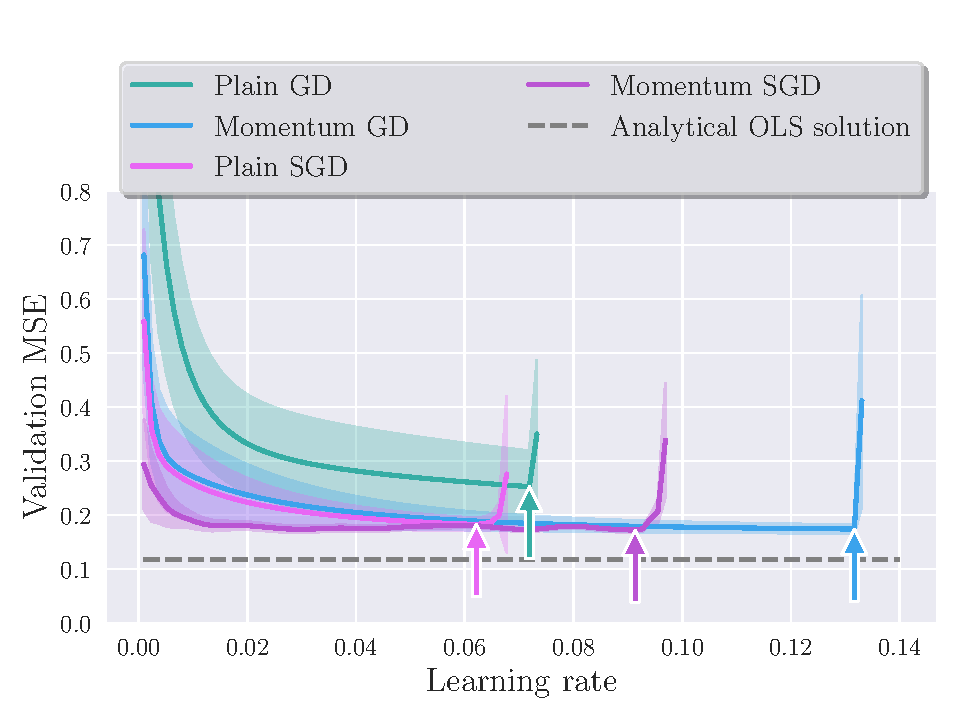
\includegraphics[width=\linewidth]{learning_rates_PGD_MGD_PSGD_MSGD.pdf}
                \caption{The minimal MSEs by algorithm: plain GD 0.1982 ($\eta=0.072$), GD w/momentum 0.1775 ($\eta=0.13$), plain SGD 0.1862 ($\eta=0.069$), SGD w/momentum 0.1729 ($\eta=0.12$)}
                \label[fig]{res:fig:lrate1}
            \end{subfigure}
            \hfill
            \begin{subfigure}{.49\textwidth}
                \centering
                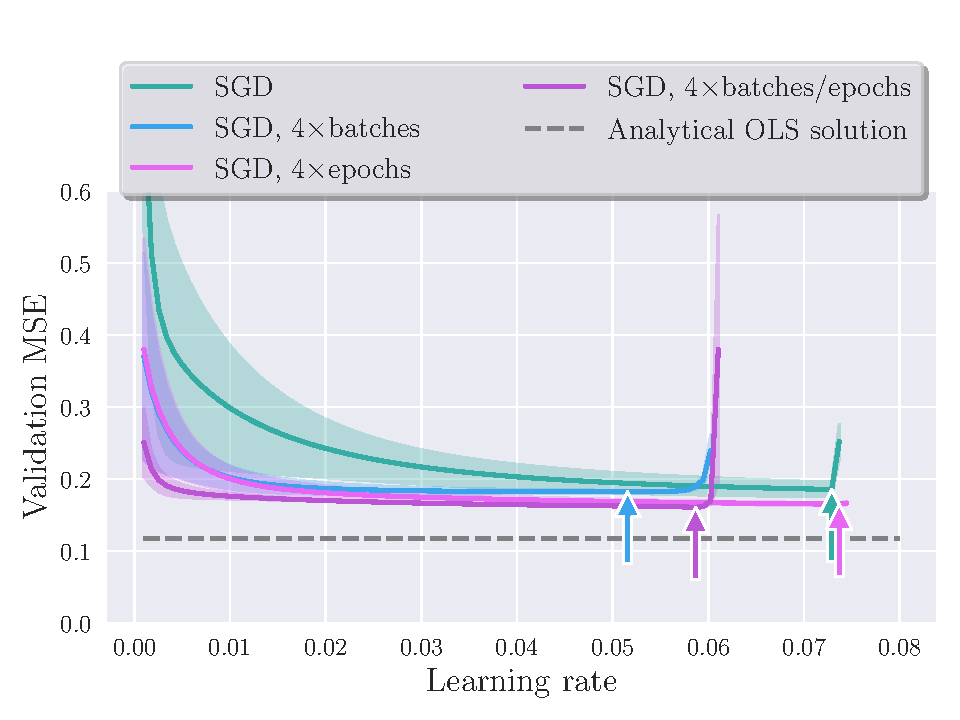
\includegraphics[width=\linewidth]{learning_rates_SGD_batches_epochs.pdf}
                \caption{The minimal MSEs of plain SGD by number of epochs and batch size: 500 epochs/200 batch size 0.1862 ($\eta=0.068$), 500 epochs/50 batch size 0.1819 ($\eta=0.0026$), 2000 epochs/64 batch size 0.1776 ($\eta=0.071$), 2000 epochs/50 batch size 0.1773 ($\eta=0.057$)}
                \label[fig]{res:fig:lrate2}
            \end{subfigure}
            \hfill
            \begin{subfigure}{.49\textwidth}
                \centering
                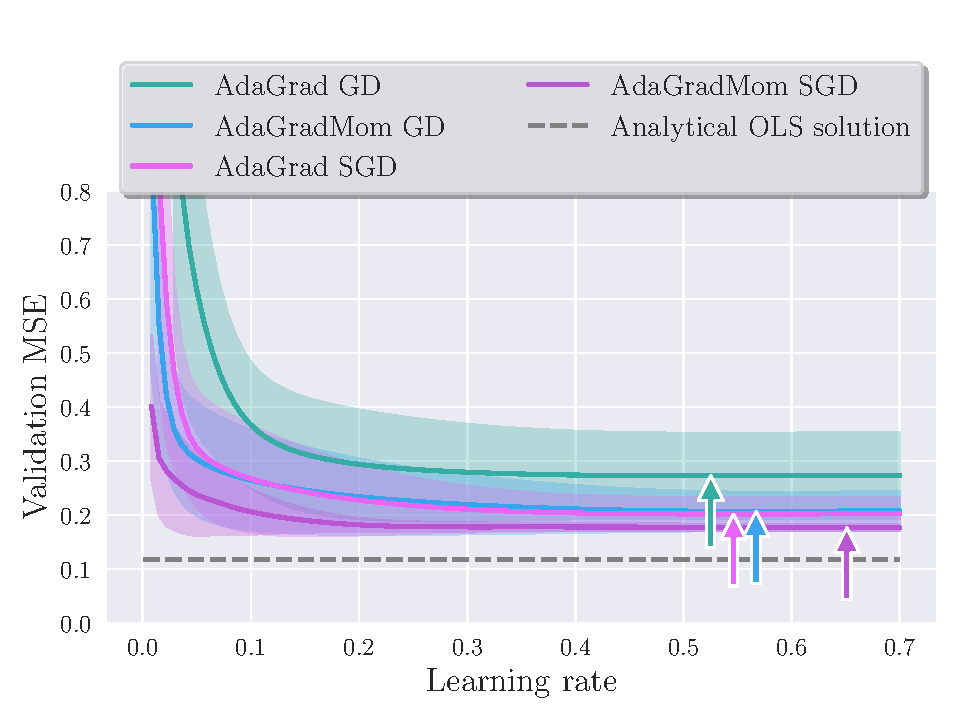
\includegraphics[width=\linewidth]{learning_rates_adagrad}
                \caption{The minimal MSEs by algorithm: AdaGrad GD 0.2135 ($\eta=0.50$), AdaGrad GD w/momentum 0.1836 ($\eta=0.52$), AdaGrad SGD 0.1906 ($\eta=0.50$), AdaGrad SGD w/momentum 0.1822 ($\eta=0.47$)}
                \label[fig]{res:fig:lrate3}
            \end{subfigure}
            \hfill
            \begin{subfigure}{.49\textwidth}
                \centering
                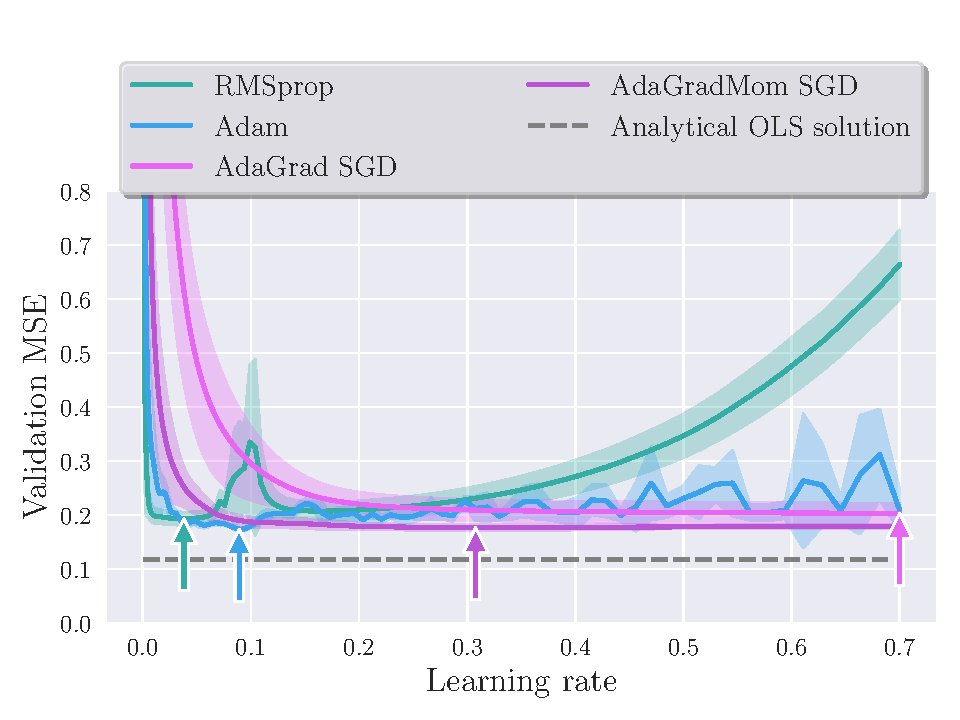
\includegraphics[width=\linewidth]{learning_rates_tunable}
                \caption{The minimal MSEs by algorithm: RMSprop SGD 0.1859 ($\eta=0.019$), Adam SGD 0.1660 ($\eta=0.32$), AdaGrad SGD 0.1906 ($\eta=0.50$), AdaGrad SGD w/momentum 0.1823 ($\eta=0.46$)}
                \label[fig]{res:fig:lrate4}
            \end{subfigure}
            \caption{Plots of the validation MSE of the parameters found from optimising the OLS cost function on Franke function data with $n=600$ data points with a train test split of $\sfrac{3}{4}$. For the momentum methods we used $\gamma=0.8$, for RMSprop we used $\beta=0.9$ and for Adam we used $\beta_1=0.9, \beta_2=0.99$. The stochastic methods used a batch size of 200 and 500 epochs, while the standard GD did 500 iterations unless specified otherwise. Overlaid are 95\% confidence intervals based on optimising with five different starting points. Exploded gradients are clipped out of the plot. The analytical OLS solution achieved an MSE of 0.1377.}
            \label[fig]{res:fig:lrates}
        \end{figure*}

    \subsubsection{Ridge Optimisation}
        The results from the ridge analysis are found in \cref{res:fig:GDridge}, and a summary is tabulated in \cref{res:tab:ridge_MSEs}. 
        
        We did not see much change in the performance of the algorithms from the OLS optimisation. There was in fact a slight decrease in the optimal MSE of all the algorithms except AdaGrad with momentum, however, the std of the MSEs generally went down. There was no universal $\lambda$-value that gave the best results. It is worth noting that there was little effect on where the exploding gradients occur; in fact with larger $\lambda$-values they occur earlier for both GD and SGD with momentum.

        The best performing algorithm was again SGD with Adam to tune the learning rate (MSE of $0.1673 \pm 0.0020$), as before with the OLS cost function.

        To see whether ridge actually had the potential to do a difference, we plotted the validation MSE of the analytical ridge solution as a function $\lambda$ against the analytical OLS solution in \cref{res:fig:ridge_ana}. We see that the ridge solution does actually perform better than OLS between $\lambda \in [0.0001, 0.01]$, meaning that there is potential for improvement with the ridge penalisation.

        \begin{table}[ht!]
            \centering
            \begin{tabular}{r|c|l|l}
                Method & MSE & $\eta$ & $\lambda$ \\ \hline
                Analytic & 0.1338 & - & 0.002 \\
                Momentum GD & $0.1777 \pm 0.0025$ & 0.13 & $10^{-4}$ \\
                Momentum SGD & $0.1747 \pm 0.0020$ & 0.12 & $10^{-8}$ \\
                AdaGrad Momentum SGD & $0.1822 \pm 0.0013$ & 0.48 & $10^{-3}$ \\
                Adam SGD & $0.1673 \pm 0.0020$ & 0.32 & $10^{-5}$
            \end{tabular}
            \caption{Summary of the best validation MSEs resulting from the optimisation of the ridge cost function using various GD algorithms. The data is taken from the plots in \cref{res:fig:GDridge}.}
            \label[tab]{res:tab:ridge_MSEs}
        \end{table}

        \begin{figure*}
            \begin{subfigure}{.49\textwidth}
                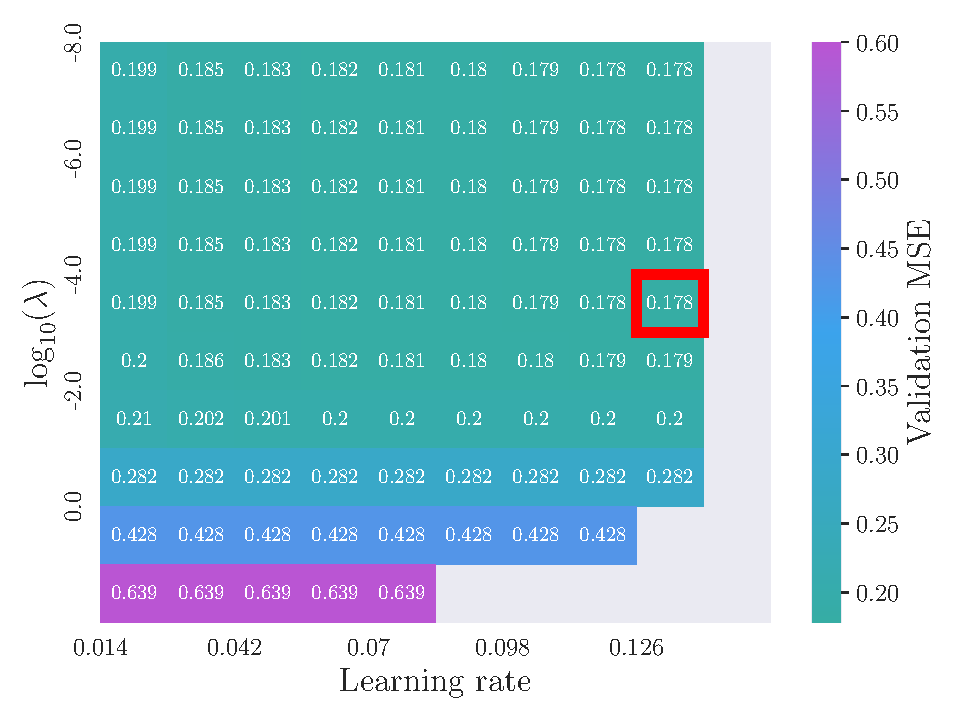
\includegraphics[width=\linewidth]{lmbda_learning_rates_momentum_GD.pdf}
                \caption{\textbf{GD with momentum}. Best MSE value was 0.1777 with $\lambda=10^{-4}, \eta=0.13$.}
                \label[fig]{res:fig:mGDridge}
            \end{subfigure}
            \hfill
            \begin{subfigure}{.49\textwidth}
                \centering
                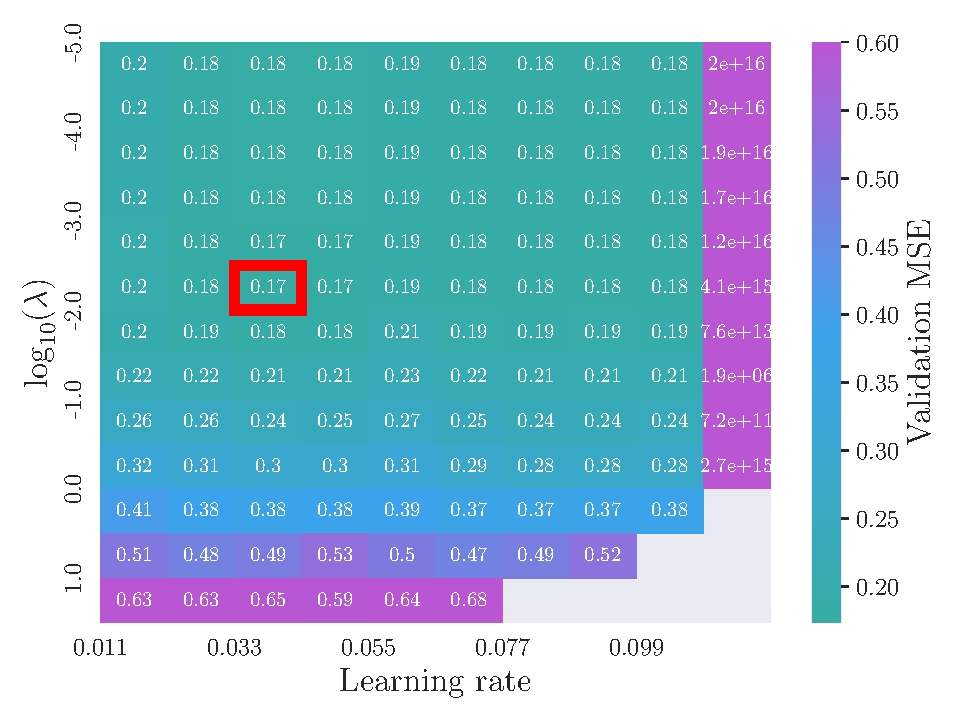
\includegraphics[width=\linewidth]{lmbda_learning_rates_momentum_SGD.pdf}
                \caption{\textbf{SGD with momentum}. Best MSE value was 0.1747 with $\lambda=10^{-8}, \eta=0.12$.}
                \label[fig]{res:fig:mSGDridge}
            \end{subfigure}
            \hfill
            \begin{subfigure}{.49\textwidth}
                \centering
                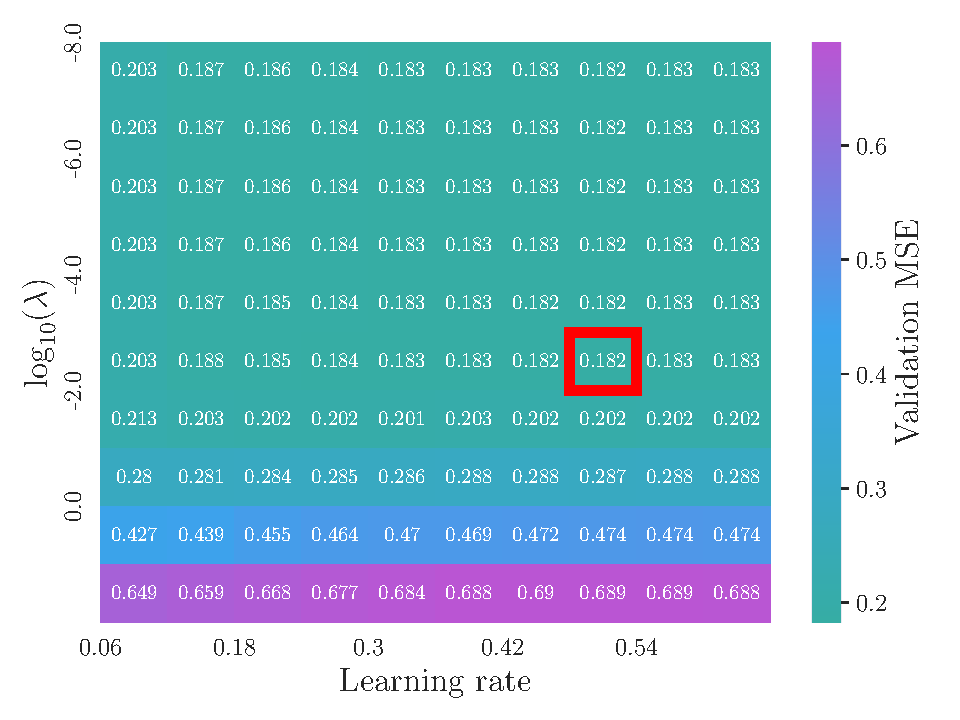
\includegraphics[width=\linewidth]{lmbda_learning_rates_adagrad_momentum_SGD.pdf}
                \caption{\textbf{SGD AdaGrad with momentum}. Best MSE value was 0.1822 with $\lambda=10^{-3}, \eta=0.48$.}
                \label[fig]{res:fig:agSGDridge}
            \end{subfigure}
            \hfill
            \begin{subfigure}{.49\textwidth}
                \centering
                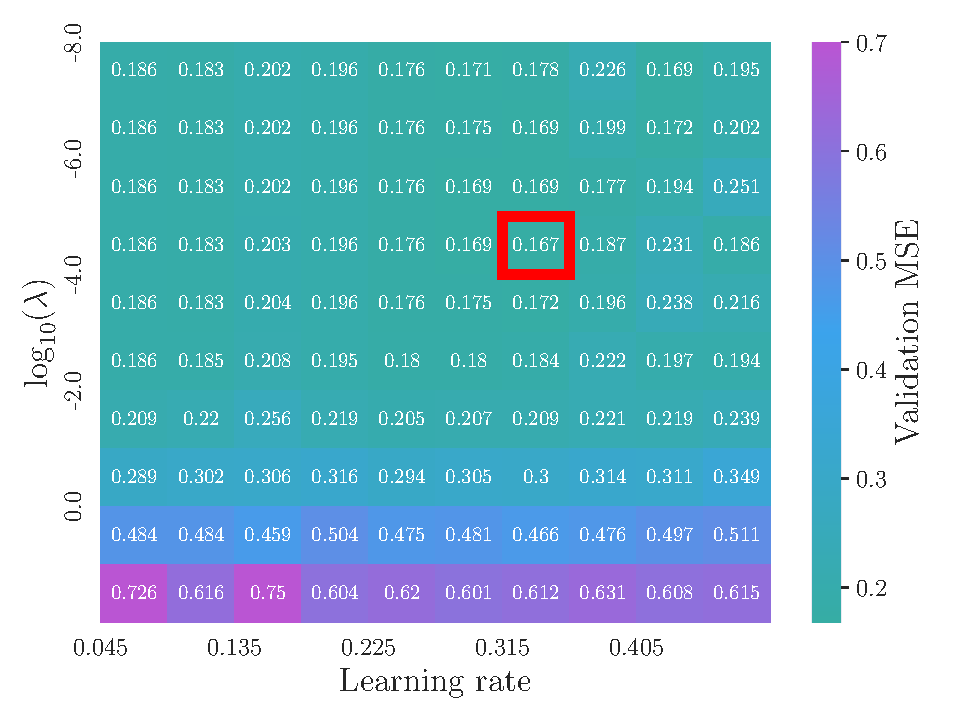
\includegraphics[width=\linewidth]{lmbda_learning_rates_adam_SGD.pdf}
                \caption{\textbf{SGD Adam}. Best MSE value was 0.1673 with $\lambda=10^{-5}, \eta=0.32$.}
                \label[fig]{res:fig:adSGDridge}
            \end{subfigure}
            \caption{Plots of the validation MSE of the parameters found from optimising the ridge cost function on Franke function data with $n=600$ data points with a train test split of $\sfrac{3}{4}$. For the momentum methods we used $\gamma=0.8$ and for Adam we used $\beta_1=0.9, \beta_2=0.99$. The stochastic methods used a batch size of 200 and 500 epochs, while the standard GD did 500 iterations unless specified otherwise. Overlaid are 95\% confidence intervals based on optimising with five different starting points. Exploded gradients are clipped out of the plot.}
            \label[fig]{res:fig:GDridge}
        \end{figure*}

        \begin{figure}[ht!]
            \centering
            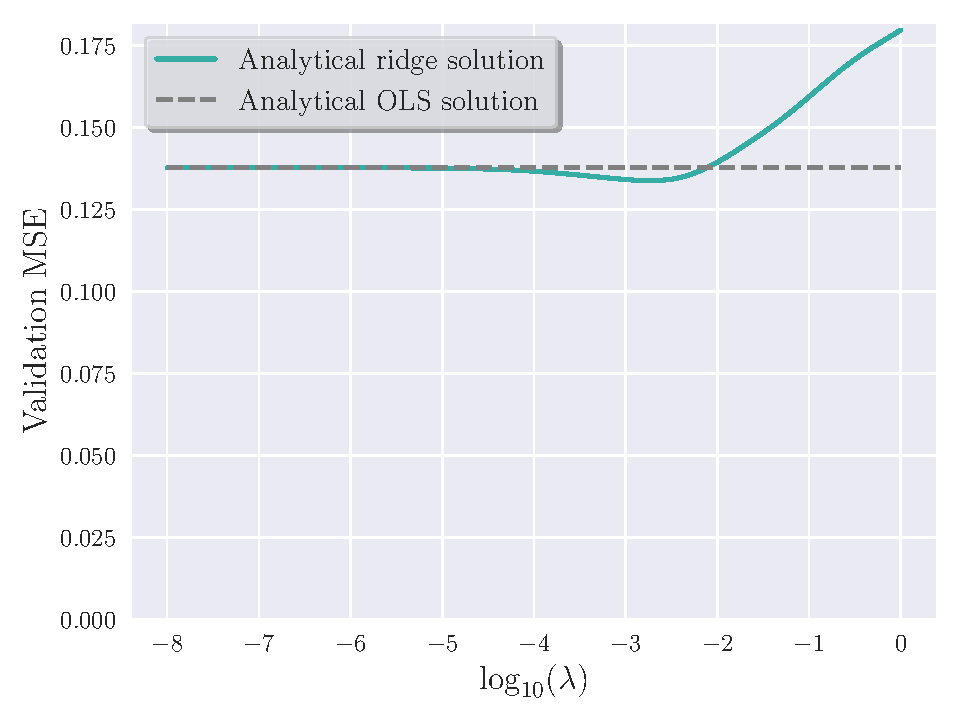
\includegraphics[width=\linewidth]{lmbda_plot_ana}
            \caption{Plot of the validation MSE found from optimising our linear regression parameters to the ridge cost function as a function of the penalisation parameter $\lambda$. The optimal MSE is 0.1338 with $\lambda = 0.002$.}
            \label[fig]{res:fig:ridge_ana}
        \end{figure}


\subsection{Wisconsin Breast Cancer}
    \begin{figure*}
        \begin{subfigure}{.49\textwidth}
            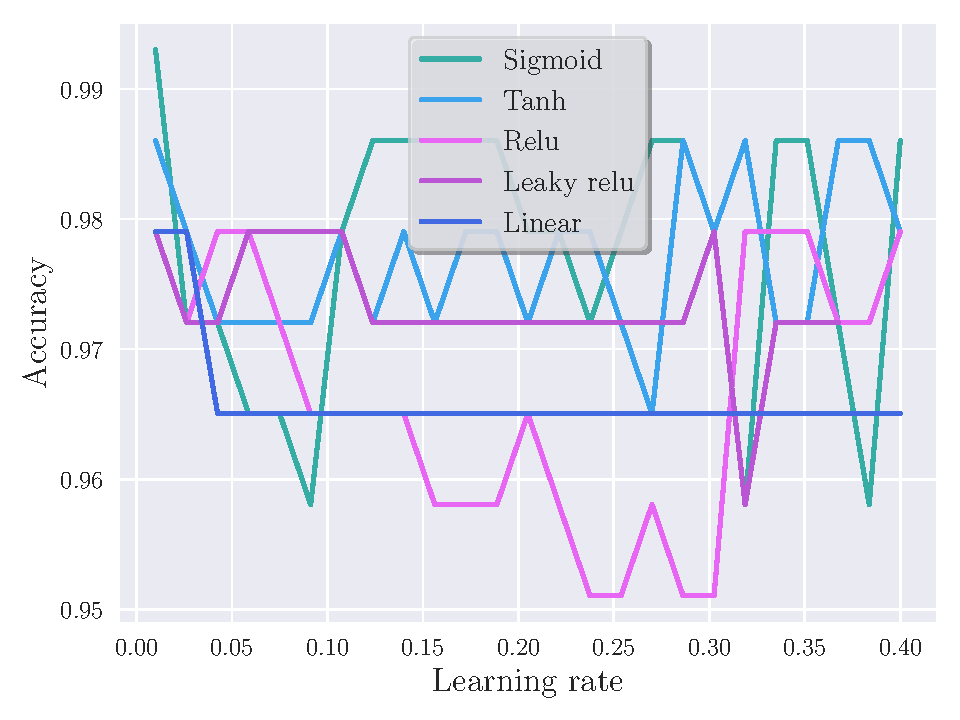
\includegraphics[width=\linewidth]{clasf_activation_functions1.pdf}
            \caption{$\eta \in [ 0.01, 0.4 ]$ with $n = 50$ points. One hidden layer with a single node}
            \label[fig]{res:fig:a}
        \end{subfigure}
        \hfill 
        \begin{subfigure}{.49\textwidth}
            \centering
            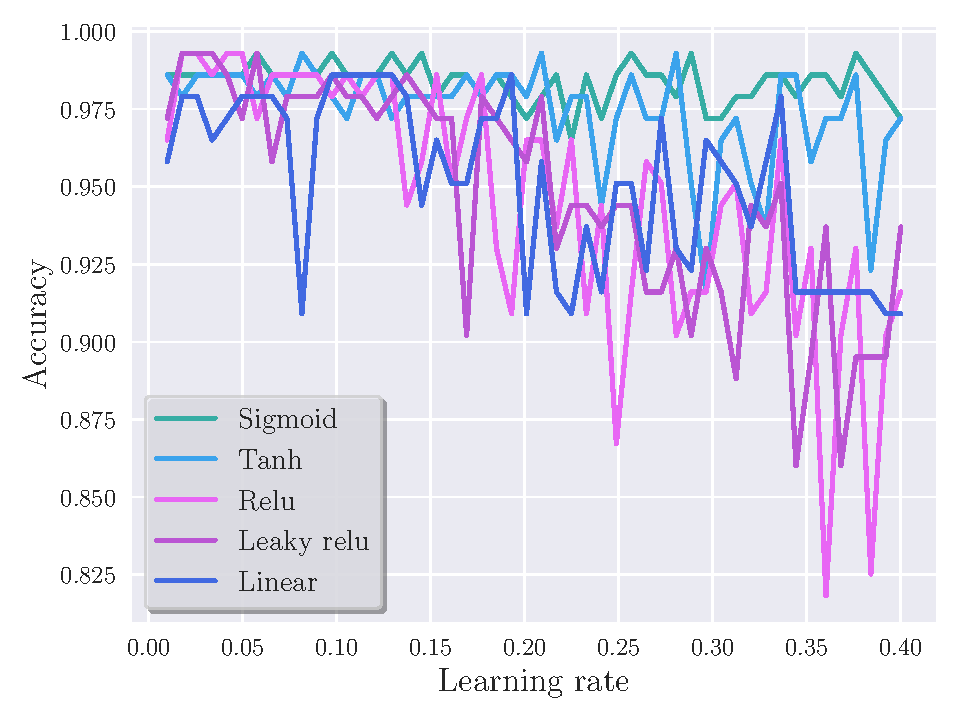
\includegraphics[width=\linewidth]{clasf_activation_functions2.pdf}
            \caption{$\eta \in [ 0.001, 0.01 ]$ with $n = 50$ points. One hidden layer 30 nodes}
            \label[fig]{res:fig:b}
        \end{subfigure}
        \hfill 
        \begin{subfigure}{.49\textwidth}
            \centering
            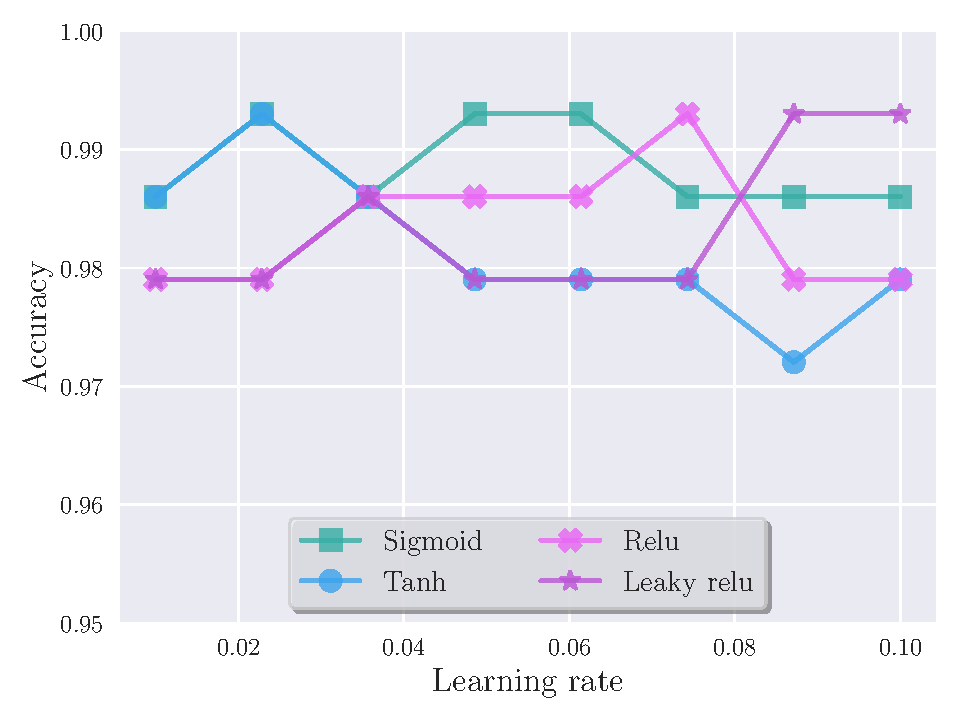
\includegraphics[width=\linewidth]{clasf_activation_functions3.pdf}
            \caption{$\eta \in [ 0.001, 0.01 ]$ with $n = 50$ points. Two hidden layers with 15 nodes each}
            \label[fig]{res:fig:c}
        \end{subfigure}
        \hfill 
        \begin{subfigure}{.49\textwidth}
            \centering
            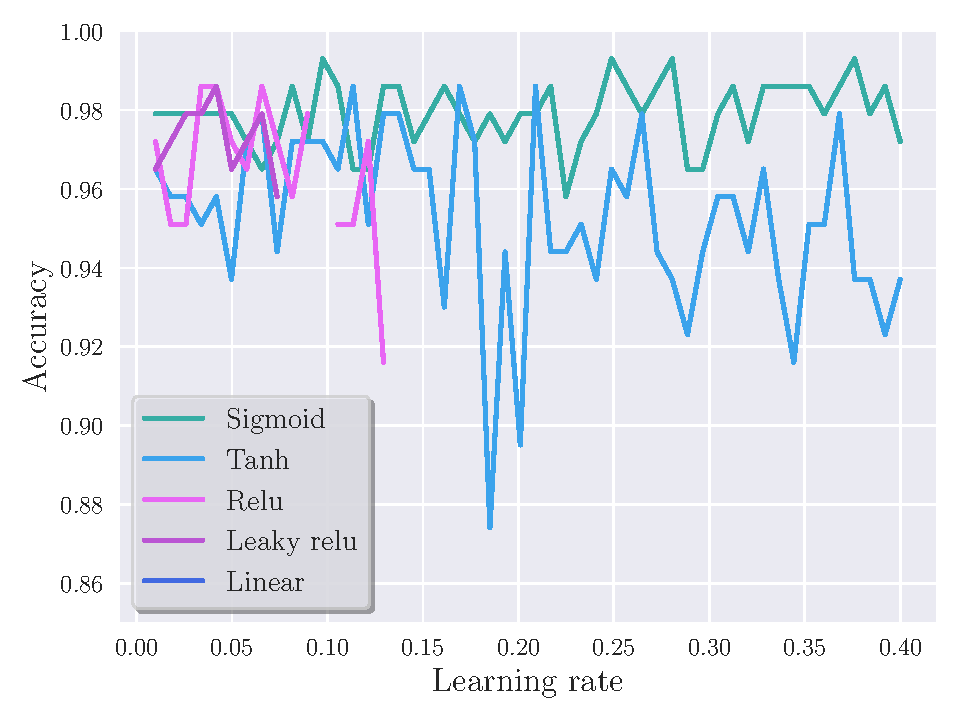
\includegraphics[width=\linewidth]{clasf_activation_functions4.pdf}
            \caption{$\eta \in [ 0.001, 0.01 ]$ with $n = 50$ points. Three hidden layers with ten nodes each}
            \label[fig]{res:fig:d}
        \end{subfigure}
    \end{figure*}

\section{Discussion}
Discussion here, in present/past tense.


\subsection{Link to existing research}
    \comment{Compare with other LWTA on MNIST and Cifar10 \Carl}
    \comment{Maybe include discussion on ML as a tool in neurobiological research \Anna} 


\subsection{Overfitting}
    \comment{I thought it would be fitting (haha) with a separate discussion on overfitting and the various ways in which we have combatted it here. -\Carl}


\subsubsection{Interpretation of pathways}
    \comment{\Anna or \Carl}

\subsubsection{Only 49 hyperparameter points explored}
    Our motivation was not to explore all of the hyperparameter space, but rather explore some structures in the high performing models. (eg. structures: MO vs CO vs Dense, and how many layer)
    \comment{\Carl or \Anna}

\section{Concluding remarks} 
Conclusion here


% for numbering appendix equations more appropriately
\numberwithin{equation}{section}
\renewcommand{\theequation}{\thesection.\arabic{equation}}
\newpage
\begin{appendices}
    \section{First Appendix}
\comment{Just add extra task things here, do not know where to put them}
\begin{figure}[H]
    \centering
    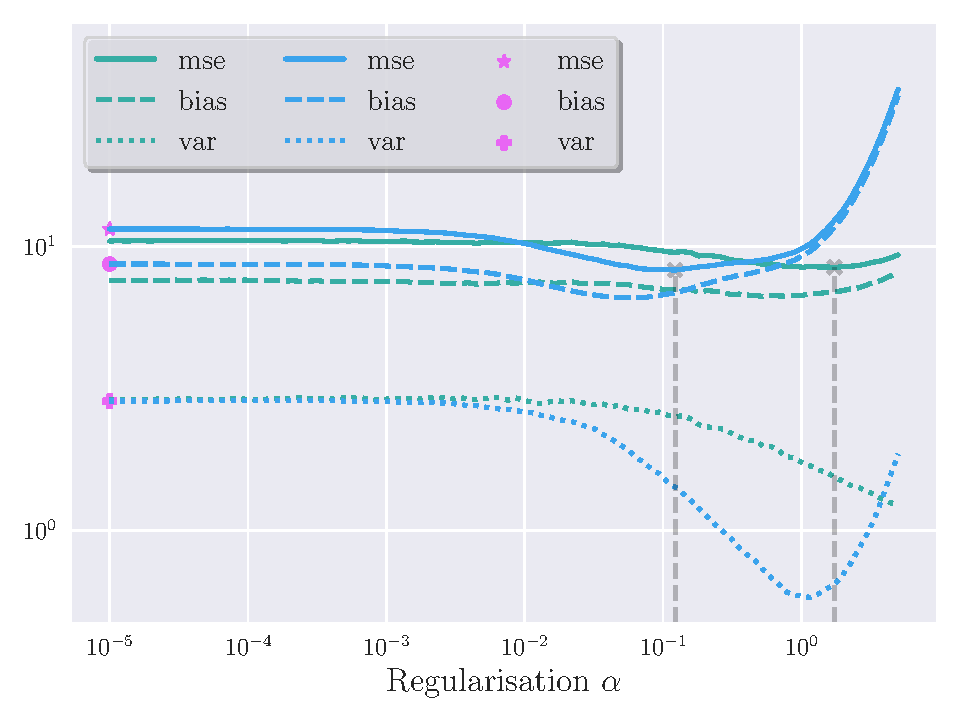
\includegraphics[width=\linewidth]{BiasVar_LinearRegression.pdf}
    \caption{MSE, bias and variance estimates for OLS (pink), Ridge (green) and Lasso (blue) as a function of regularisation parameter $\alpha$.}
    \label[fig]{fig:linreg_biasvar_decomp}
\end{figure}

\begin{figure}[H]
    \centering
    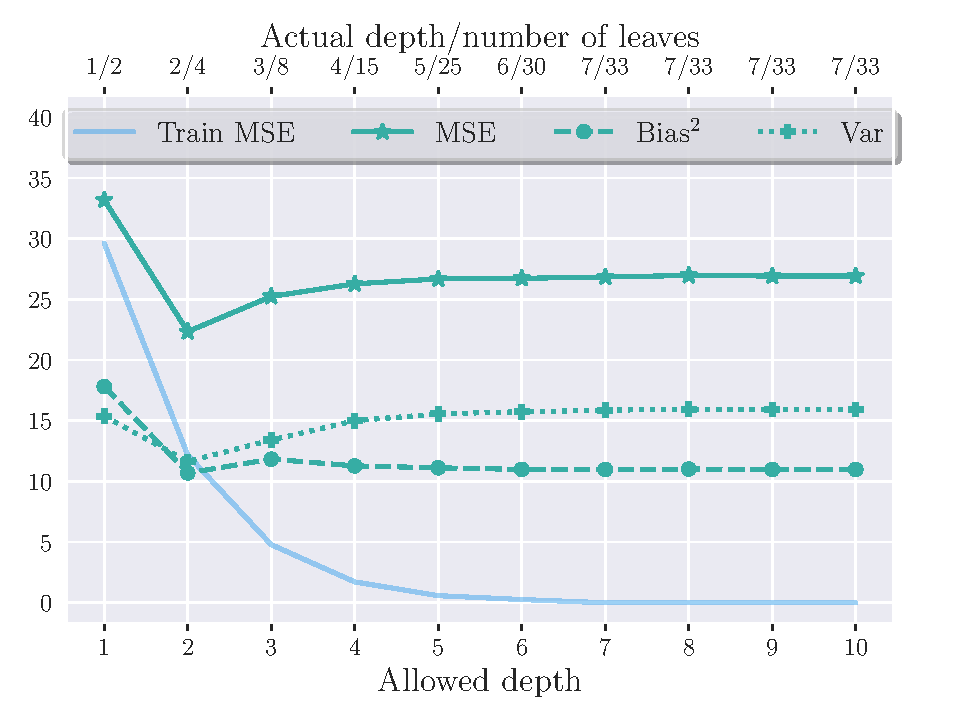
\includegraphics[width=\linewidth]{BiasVar_SingleTree.pdf}
    \caption{MSE, bias and variance estimates for a single tree against increasing relaxation of tree depth.}
    \label[fig]{fig:singletree_biasvar_decomp}
\end{figure}
 
\end{appendices}

% \printbibliography
\bibliography{refs/references}

\end{document}

